\documentclass[final,5p,times,twocolumn]{elsarticle}

\usepackage{amsmath}
\usepackage{amssymb}
\usepackage{graphicx}
\usepackage{booktabs}
\usepackage{tabularx}
\usepackage{multirow}
\usepackage[hidelinks]{hyperref}
\usepackage{siunitx}
\sisetup{detect-all, group-separator = {,}, group-minimum-digits = 4,
  group-digits = integer, range-phrase = --, range-units = single,
  list-units = single}
\DeclareSIUnit{\MW}{MW}
\DeclareSIUnit{\MWh}{MWh}
\DeclareSIUnit{\MVA}{MVA}
\DeclareSIUnit{\MVAr}{MVAr}

\graphicspath{{figures/}}

\setcounter{topnumber}{3}
\setcounter{bottomnumber}{2}
\setcounter{totalnumber}{5}
\setcounter{dbltopnumber}{3}
\renewcommand{\topfraction}{0.92}
\renewcommand{\dbltopfraction}{0.92}
\renewcommand{\bottomfraction}{0.5}
\renewcommand{\textfraction}{0.08}
\renewcommand{\floatpagefraction}{0.70}
\renewcommand{\dblfloatpagefraction}{0.70}

\newcommand{\pu}{\ensuremath{\mathrm{pu}}}
\newcommand{\yes}{\ensuremath{\bullet}}
\newcommand{\no}{\ensuremath{\circ}}

\journal{Sustainable Energy, Grids and Networks}

\begin{document}

\begin{frontmatter}

\title{Current-limited capability of grid-forming converters in reserve and
inertia scheduling: formulation, sign condition and validation}

\author[hyu]{Junseok Lim}
\author[hyu]{Sanghyuk Ji}
\author[hyu]{Byungjun Lee}
\author[hyu]{Sungwoo Bae\corref{cor1}}
\ead{swbae@hanyang.ac.kr}
\cortext[cor1]{Corresponding author.}
\address[hyu]{Department of Electrical Engineering, Hanyang University,
Seoul, Republic of Korea}

\begin{abstract}
Scheduling formulations in which energy, reserve and inertia share the
capability of a grid-forming converter bound that capability by active power
and omit the current limit that couples the three services. This paper
represents the continuous and short-term current ratings, reactive current
and terminal voltage of the converter as a polyhedral capability set and
integrates it in a multi-period linear clearing whose prices are dual
variables. A piecewise condition is derived for the sign of the error made by
the active-power bound; it depends on the short-term current radius, the
bound and the reactive current held during the response. Final schedules on
the IEEE 39-bus and RTS-24 systems are obtained by successive linearisation
and satisfy bus voltage, generator reactive, branch loading and balance
limits in an ac power flow for both representations. The procured response
is constrained to be deliverable after the largest generator outages, and a
current-limited RMS converter model confirms that the scheduled inertial
power is delivered within the current limit at the terminal voltage reached
during the event. The three omissions change the cleared cost with different
signs, so a constant derating cannot correct the bound. Across four rating
conventions, two bound definitions, three comparison models and 605
randomised converter placements, the capability set is never the more
expensive representation. The cost difference is 0.3 to 1.1\,\% at the base
case and depends on the rating convention; the inertia price under the
active-power bound is 2.3 to 13.7 times that under the capability set.
\end{abstract}

\begin{keyword}
grid-forming converter \sep inertia \sep operating reserve \sep
capability curve \sep ancillary service pricing \sep converter current limit
\end{keyword}

\end{frontmatter}

\begin{table*}[t]
  \section*{Nomenclature}
  \centering
  \small
  \begin{tabular*}{\textwidth}{@{\extracolsep{\fill}}l l l l@{}}
    \toprule
    $i$, $g$, $t$, $z$, $\omega$ & converter, synchronous unit, period, zone,
      outage
      & $P_i$, $Q_i$, $\tilde{Q}_i$ & active, reactive, short-term reactive
      power \\
    $S_i$, $P^{\mathrm{sch}}_i$, $\bar{P}_i$ & rating, scheduled active
      bound, comparison bound
      & $R_i$, $H_i$ & reserve, inertial power (MW) \\
    $I^{\mathrm{c}}$, $I^{\mathrm{s}}$ & continuous, short-term current limit
      (pu)
      & $p^{\mathrm{d}}$, $p^{\mathrm{c}}$, $c$, $e$ & discharge, charge,
      curtailment, available injection \\
    $V_i$, $V^{\mathrm{sh}}_i$ & pre-event, event terminal voltage (pu)
      & $a_i$, $\sigma_i$ & band availability, state of charge \\
    $\alpha_i$, $\chi$ & reactive priority, reserve overlap
      & $p^{\mathrm{g}}$, $r^{\mathrm{g}}$ & synchronous energy, reserve \\
    $m$, $\beta_i$, $L_i$ & polygon faces, band width, short-term radius
      & $\lambda$, $\mu$ & energy price, requirement prices \\
    $\underline{\sigma}^{\mathrm{e}}$, $\sigma^{\star}$, $E_i$ & energy
      floor, full-band breakpoint, store energy
      & $\rho$, $\varphi$, $\dot{f}^{\max}$ & reserve, reactive requirement
      fractions, RoCoF limit \\
    $\tau^{\mathrm{R}}$, $\tau^{\mathrm{H}}$ & reserve, inertia delivery
      windows
      & $\boldsymbol{\Psi}$, $\mathbf{f}^{\max}$, $\varepsilon$ & shift
      factors, branch ratings, emergency factor \\
    $\mathcal{H}_g$, $S_g$ & inertia constant (s), rating of unit $g$
      & $\delta$, $\tilde{Q}^{\mathrm{crit}}$ & cost difference, crossing of
      the Proposition \\
    $\kappa^{\bullet}$ & offers
      & $x^{\mathrm{g}}_i$, $\phi^t_\omega$ & reactance behind terminal,
      deployed fraction \\
    $\gamma^{\mathrm{UD}}$, $\kappa^{\mathrm{Q}}$ & uniform derating factor,
      reactive range
      & $\mathcal{I}$, $\mathcal{G}$, $\mathcal{Z}_{\mathcal{I}}$ & converters,
      synchronous units, zones with converters \\
    \bottomrule
  \end{tabular*}
\end{table*}

% Sections 1--3 of the revised manuscript (r2, six-section structure:
% 1 Introduction, 2 Capability set and sign condition, 3 Market clearing
% formulation, 4 Case study, 5 Results, 6 Conclusion). Numbers that depend on the
% regenerated results are marked \todo{...} and filled from study/results.

\section{Introduction}
\label{sec:intro}

As synchronous generation is displaced, inertia and fast reserve have to be
procured explicitly, and increasingly from converter-interfaced
resources~\cite{ulbig2014inertia,tielens2016inertia,milano2018lowinertia}.
Grid-forming (GFM) control, in which the converter behaves as a voltage source
behind an impedance, is the main technical
response~\cite{zhong2011synchronverter,rocabert2012control,dorfler2023control},
and system operators now specify GFM capability rather than encourage
it~\cite{matevosyan2019gfm,lin2020roadmap,entsoe2020gfm}. The energy a GFM
converter sells, the reserve it holds and the inertial power it injects after
a disturbance all pass through the same semiconductor bridge, so they are
limited jointly, and the limit is a current~\cite{yazdani2010vsc}.

Scheduling formulations have treated the frequency side of this problem in
increasing detail. Governor rate limits entered the optimal power flow
in~\cite{chavez2014governor}; inertia became a decision variable
in~\cite{teng2016stochastic}; frequency services were
co-optimised in~\cite{badesa2019simultaneous,trovato2019unit}; and
requirement uncertainty and the siting of virtual inertia were addressed
in~\cite{paturet2020stochastic,poolla2019placement}. On the supply side these
models bound what a resource can offer by active power. Three recent
formulations require converter inertia to be backed by unused
headroom~\cite{park2026inertia,jiang2025frequency,beigifard2026frequency},
and a fourth embeds a learned frequency surrogate in the day-ahead
schedule~\cite{jiang2026learning}. They differ in most respects, but in each
the converter capability has the form
%
\begin{equation}
  P_i + R_i + H_i \;\le\; \bar{P}_i ,
  \label{eq:box}
\end{equation}
%
with $P_i$ the energy schedule, $R_i$ the reserve and $H_i$ the inertial
power. None contains a current limit, a reactive-power term or the terminal
voltage (Table~\ref{tab:related}).

System operators describe the capability differently. AEMO specifies overload
capability as a level with a duration, for example \SI{150}{\percent} of rated
current for \SI{2}{\second}, and reports that the active headroom of an
inverter depends on its pre-disturbance operating
point~\cite{aemo2023gfm,aemo2024inertia}; MISO's draft specification addresses
operation at short-duration current limits~\cite{miso2024gfm}. At device and
feeder level the interaction between reactive support and active reserve
through the apparent-power limit is
established~\cite{energies2020reserve}, and current-based inverter limits
have been used in photovoltaic--storage scheduling and in batteries providing
frequency and voltage control
together~\cite{polat2025inverter,zecchino2021concurrent}. The remaining gap is
a market clearing in which the current limit is shared between energy, reserve
and inertia, the requirement multipliers are prices, and the effect of the
representation is quantified.

\begin{table*}[t]
  \caption{Scheduling formulations with shared converter capability and what
  each represents ($\yes$ present, $\no$ absent, --- not applicable). Entries
  follow the constraint sets stated in each paper.}
  \label{tab:related}
  \centering
  \footnotesize
  \begin{tabular*}{\textwidth}{@{\extracolsep{\fill}}l l c c c c c c c l@{}}
    \toprule
    & & Shared & Current & Reactive & Terminal & Short-term
    & Storage & Prices & Frequency \\
    Reference & Test system & capability & limit & power & voltage
    & $\neq$ continuous & state & as duals & model \\
    \midrule
    Park et al.~\cite{park2026inertia} & IEEE 30
      & \yes & \no & \no & \no & \no & \yes & \yes & --- \\
    Jiang and Li~\cite{jiang2025frequency} & WSCC 9, IEEE 39
      & \yes & \no & \no & \no & \no & \no & \no & EMT surrogate \\
    Jiang and Li~\cite{jiang2026learning} & IEEE 9
      & \yes & \no & \no & \no & \no & \yes & \no & EMT surrogate \\
    Beigi Fard et al.~\cite{beigifard2026frequency} & IEEE 9, 118
      & \yes & \no & \no & \no & \no & \yes & \no & PWL nadir \\
    Garozzo and Tina~\cite{energies2020reserve} & inverter, LV feeder
      & --- & \yes & \yes & \no & \no & \yes & --- & --- \\
    \addlinespace
    This work & IEEE 39, RTS-24
      & \yes & \yes & \yes & \yes & \yes & \yes & \yes & RMS check \\
    \bottomrule
  \end{tabular*}
\end{table*}

The physical limit on a converter is
%
\begin{equation}
  \sqrt{P^2 + Q^2} \;\le\; V I_{\max} S ,
  \label{eq:disc}
\end{equation}
%
a disc in the $P$--$Q$ plane whose radius scales with the terminal voltage
$V$. Equation~\eqref{eq:box} is the projection of Eq.~\eqref{eq:disc} onto
$Q = 0$ at $V = \SI{1.0}{\pu}$ with $I_{\max}$ fixed at the continuous rating.
It therefore omits the short-term current rating, which understates the
capability available for an inertial response; omits reactive current, which
overstates capability whenever $Q \neq 0$; and fixes the voltage, which
overstates capability below \SI{1.0}{\pu} and understates it above. The three
errors do not have the same sign, so a constant derating of
Eq.~\eqref{eq:box} cannot remove them together.

The contributions of this paper are as follows.
\begin{enumerate}
  \item The continuous and short-term current ratings, reactive current and
        terminal voltage of a GFM converter are represented as a polyhedral
        capability set and integrated in a multi-period joint clearing of
        energy, reserve and inertia with marginal pricing. The clearing
        remains a linear programme, so the prices are dual variables.
  \item A piecewise condition is derived for the sign of the error made by
        the active-power bound of Eq.~\eqref{eq:box}. The condition depends
        on the short-term radius, the bound and the reactive current held
        during the response, and not on the sustained active power.
  \item The formulation is evaluated on the IEEE 39-bus and RTS-24 systems
        against three comparison models and an exact second-order cone
        benchmark, under alternative converter rating conventions and
        randomised converter placements. The final schedules are validated
        by ac power flow against voltage, generator reactive, branch and
        balance limits; the procured response is constrained to be
        deliverable after the largest generator outages; and the scheduled
        inertial power is checked against a current-limited RMS converter
        model.
\end{enumerate}

Fig.~\ref{fig:overview} summarises the approach. The formulation extends the
shared-capability clearing of~\cite{park2026inertia}, whose treatment of
inertia as a priced power service and of storage energy recovery is retained;
what changes is the shape of the set the services share.

\begin{figure*}[t]
  \centering
  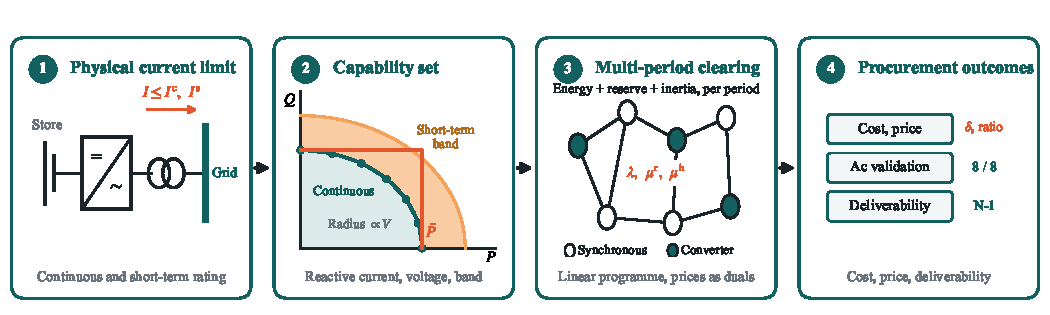
\includegraphics[width=\textwidth]{fig1_overview}
  \caption{Overview: physical current limit, polyhedral capability set,
  multi-period clearing with network and ac validation, and procurement
  outcomes.}
  \label{fig:overview}
\end{figure*}

\section{Capability set and sign condition}
\label{sec:capability}

\subsection{Continuous and short-term limits}

Converter $i$ has apparent-power rating $S_i$, terminal voltage $V_i$ (pu),
continuous current limit $I^{\mathrm{c}}$ and short-term current limit
$I^{\mathrm{s}} \ge I^{\mathrm{c}}$ (pu of rated current). Reserve that is
called must be sustained for the containment period, whereas the inertial
response lasts of the order of a second. Two constraints follow:
%
\begin{align}
  \sqrt{(P_i + R_i)^2 + Q_i^2} &\;\le\; V_i I^{\mathrm{c}} S_i ,
  \label{eq:cont} \\
  \sqrt{(P_i + \chi R_i + H_i)^2 + \tilde{Q}_i^2}
    &\;\le\; V^{\mathrm{sh}}_i \big[ I^{\mathrm{c}}
      + a_i (I^{\mathrm{s}} - I^{\mathrm{c}}) \big] S_i .
  \label{eq:short}
\end{align}
%
Equation~\eqref{eq:cont} applies the continuous (thermal) rating to the
sustained schedule. It is imposed at both ends of the reserve activation,
$(P_i, Q_i)$ and $(P_i + R_i, Q_i)$, because a charging converter
($P_i < 0$) carries its largest current before its reserve is called; the set
is convex, so the intermediate points are covered.
Equation~\eqref{eq:short} applies the short-term rating at the instant of the
inertial response. The factor $\chi \in [0,1]$ is the fraction of the reserve
already activated at that instant and is set to one, the simultaneous
envelope. $V^{\mathrm{sh}}_i$ is the terminal voltage during the event; it
equals $V_i$ unless the correction of Section~\ref{sec:applied} is applied.
The band availability $a_i \in [0,1]$ is defined below.
Fig.~\ref{fig:capability} compares the two constraints with
Eq.~\eqref{eq:box}.

\begin{figure}[t]
  \centering
  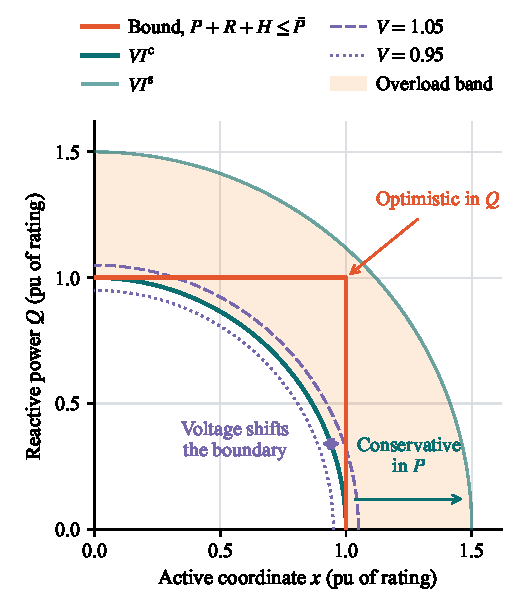
\includegraphics[width=\columnwidth]{fig2_capability}
  \caption{Capability set and active-power bound at
  $I^{\mathrm{c}} = \SI{1.0}{\pu}$, $I^{\mathrm{s}} = \SI{1.5}{\pu}$.}
  \label{fig:capability}
\end{figure}

\subsection{Reactive current priority}

During a short-term excursion the current-priority setting of the converter
determines how much reactive current is
retained~\cite{qoria2020current,bottrell2014comparison}. The setting is a
property of the converter, so it enters as a parameter:
%
\begin{equation}
  \tilde{Q}_i = \alpha_i Q_i , \qquad \alpha_i \in [0,1] ,
  \label{eq:priority}
\end{equation}
%
with $\alpha_i = 1$ for reactive priority and $\alpha_i = 0$ for ideal active
priority. Writing the relation as a bound $0 \le \tilde{Q}_i \le Q_i$ would
let the optimisation choose the converter's current allocation.

\subsection{Storage state of charge}

A store limits the services in two ways. The short-term band is available
only above an energy floor $\underline{\sigma}^{\mathrm{e}}$ and fully
available above a breakpoint $\sigma^{\star}$,
%
\begin{equation}
  0 \;\le\; a_i^t \;\le\; \min\!\left(1, \;
    \frac{\min\!\left(\sigma_i^{t-1}, \sigma_i^{t}\right)
      - \underline{\sigma}^{\mathrm{e}}}
    {\sigma^{\star} - \underline{\sigma}^{\mathrm{e}}}\right) ,
  \label{eq:gate}
\end{equation}
%
and the energy behind the services must be held for their delivery windows
$\tau^{\mathrm{R}}$ and $\tau^{\mathrm{H}}$,
%
\begin{equation}
  \frac{\tau^{\mathrm{R}} R_i^t + \tau^{\mathrm{H}} H_i^t}{\eta_{\mathrm{d}}}
    \;\le\; \Bigl( \min\!\left(\sigma_i^{t-1}, \sigma_i^{t}\right)
      - \underline{\sigma}^{\mathrm{e}} \Bigr) E_i .
  \label{eq:deliverability}
\end{equation}
%
Both are evaluated at the two ends of the period and are linear in the state
of charge. The linear ramp in Eq.~\eqref{eq:gate} is an assumption; moving the
breakpoint $\sigma^{\star}$ across its range changes the reported cost
differences by less than \num{0.05} percentage points.

\subsection{Polyhedral form}
\label{sec:polygon-error}

Equations~\eqref{eq:cont} and~\eqref{eq:short} are second-order cones. Each
is replaced by an inscribed regular $m$-gon~\cite{bental2001polyhedral},
%
\begin{align}
  (P_i + R_i)\cos\theta_k + Q_i \sin\theta_k
    &\;\le\; V_i I^{\mathrm{c}} S_i \cos\tfrac{\pi}{m} ,
  \label{eq:polygon} \\
  (P_i + \chi R_i + H_i)\cos\theta_k + \tilde{Q}_i \sin\theta_k
    - a_i \beta_i
    &\;\le\; V^{\mathrm{sh}}_i I^{\mathrm{c}} S_i \cos\tfrac{\pi}{m} ,
  \label{eq:polygon-short}
\end{align}
%
for $\theta_k = 2\pi k / m$, $k = 0, \dots, m-1$, with
$\beta_i = V^{\mathrm{sh}}_i (I^{\mathrm{s}} - I^{\mathrm{c}}) S_i
\cos(\pi/m)$ the width of the overload band. The band width is a parameter,
so both constraints are affine. The polygon is an inner approximation: the
clearing cost is an upper bound on that of the exact conic problem. With
$m = 24$ the cleared cost exceeds the exact second-order cone solution by at
most \SI{0.066}{\percent} over the configurations of
Section~\ref{sec:results}, and by \SI{0.0045}{\percent} with $m = 96$. The case
study uses $m = 24$, and $m = 192$ where the polygon error would be comparable
to the effect measured.

\subsection{Sign of the error of the active-power bound}
\label{sec:sign}

Consider a sustained operating point admitted by both representations. The
radius allowed by the short-term constraint is
%
\begin{equation}
  L_i = V^{\mathrm{sh}}_i \big[ I^{\mathrm{c}}
        + a_i (I^{\mathrm{s}} - I^{\mathrm{c}}) \big] S_i .
  \label{eq:radius}
\end{equation}
%
The active-power bound leaves inertial headroom
$H^{\mathrm{ap}}_i = \bar{P}_i - (P_i + R_i)$ and the capability set leaves
$H^{\mathrm{set}}_i = \sqrt{L_i^2 - \tilde{Q}_i^2} - (P_i + \chi R_i)$, so
%
\begin{equation}
  \Delta H_i = H^{\mathrm{set}}_i - H^{\mathrm{ap}}_i
    = \sqrt{L_i^2 - \tilde{Q}_i^2} - \bar{P}_i + (1 - \chi) R_i .
  \label{eq:difference}
\end{equation}
%
At $\chi = 1$ the difference does not depend on the sustained active power.

\medskip
\noindent\textbf{Proposition.} Let $\chi = 1$ and $L_i$ be given by
Eq.~\eqref{eq:radius}.
\emph{(i)} If $L_i > \bar{P}_i$, define
$\tilde{Q}^{\mathrm{crit}}_i = \sqrt{L_i^2 - \bar{P}_i^2}$. The active-power
bound understates the inertial headroom for
$|\tilde{Q}_i| < \tilde{Q}^{\mathrm{crit}}_i$, is exact at
$|\tilde{Q}_i| = \tilde{Q}^{\mathrm{crit}}_i$, and overstates it for
$|\tilde{Q}_i| > \tilde{Q}^{\mathrm{crit}}_i$.
\emph{(ii)} If $L_i = \bar{P}_i$, the two agree only at $\tilde{Q}_i = 0$ and
the bound overstates elsewhere.
\emph{(iii)} If $L_i < \bar{P}_i$, the bound overstates for every admissible
$\tilde{Q}_i$.
\medskip

The proof follows from Eq.~\eqref{eq:difference}. A higher $I^{\mathrm{s}}$, a
higher voltage or a larger band availability increases $L_i$ and moves the
bound towards understatement; a larger $|\tilde{Q}_i|$ moves it towards
overstatement. The multiplier that would make Eq.~\eqref{eq:box} exact,
$\gamma_i = \sqrt{L_i^2 - \tilde{Q}_i^2} / \bar{P}_i$, varies with voltage,
reactive dispatch, short-term rating and band availability, so no constant
derating reproduces it. The quantities in the condition are available at the
time of clearing: terminal voltage from the state estimator, ratings from
equipment data and reactive dispatch from the schedule. Region (iii) applies
when $V^{\mathrm{sh}}_i I^{\mathrm{s}} < \bar{P}_i / S_i$ with the band
withdrawn, i.e.\ at low voltage with little overload capability.

Fig.~\ref{fig:signmap} gives the crossing for $\bar{P} = S$ and full
band availability. At $I^{\mathrm{s}} =
\SI{1.5}{\pu}$ the crossing exceeds the rating over the normal voltage band,
so the bound is conservative for practical reactive dispatch. At
$I^{\mathrm{s}} = \SI{1.1}{\pu}$ it lies between \num{0.30} and \num{0.58}, a
range that ordinary reactive duty reaches. The condition was checked against
the exact disc at \num{1884} points over $V \in [0.90, 1.08]$,
$I^{\mathrm{s}} \in [1.0, 1.8]$, three band availabilities and two bounds,
and gives the correct sign at all of them.

\begin{figure}[t]
  \centering
  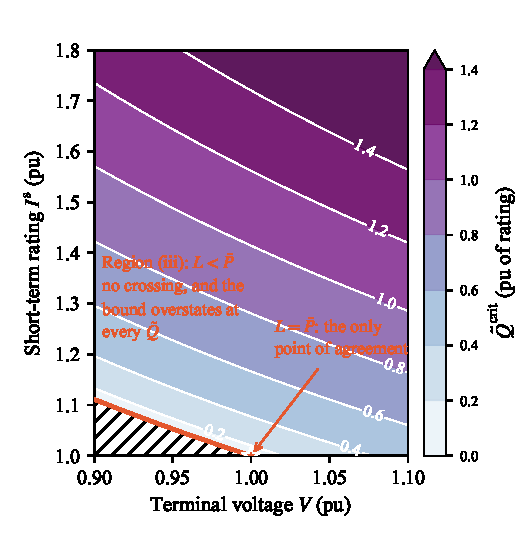
\includegraphics[width=\columnwidth]{fig3_sign_map}
  \caption{Crossing $\tilde{Q}^{\mathrm{crit}}$ (pu of rating) at
  $\bar{P} = S$ and full band availability. Below the heavy contour
  $L < \bar{P}$ and the bound overstates at every reactive dispatch.}
  \label{fig:signmap}
\end{figure}

\section{Market clearing formulation}
\label{sec:clearing}

\subsection{Objective and requirements}

The clearing covers $T$ periods of length $\Delta$ with converters $i \in
\mathcal{I}$, synchronous units $g \in \mathcal{G}$ and zones $z \in
\mathcal{Z}$. The decisions are converter discharge $p^{\mathrm{d}}$, charge
$p^{\mathrm{c}}$, curtailment $c$, reactive output $Q$, reserve $R$, inertial
power $H$, band availability $a$ and state of charge $\sigma$, and
synchronous energy $p^{\mathrm{g}}$ and reserve $r^{\mathrm{g}}$. With
$e_i^t$ the available converter injection, the net converter injection is
%
\begin{equation}
  P_i^t = e_i^t + p^{\mathrm{d},t}_i - p^{\mathrm{c},t}_i - c_i^t ,
  \label{eq:injection}
\end{equation}
%
and the objective is
%
\begin{align}
  \min \; \Delta \sum_t \Big[ & \sum_i \big( \kappa^{\mathrm{e}}
      p^{\mathrm{d},t}_i + \kappa^{\mathrm{r}} R_i^t
      + \kappa^{\mathrm{h}} H_i^t + \kappa^{\mathrm{q}} Q_i^t
      + \kappa^{\mathrm{cyc}} ( p^{\mathrm{d},t}_i + p^{\mathrm{c},t}_i )
      \big) \nonumber \\
  & + \sum_g \big( \kappa^{\mathrm{ge}} p^{\mathrm{g},t}_g
    + \kappa^{\mathrm{gr}} r^{\mathrm{g},t}_g \big) \Big] ,
  \label{eq:objective}
\end{align}
%
with energy offers in \$/MWh and availability offers in \$/MW/h. The power
balance and the reserve, inertia and zonal reactive requirements are
%
\begin{align}
  \sum_i P_i^t + \sum_g p^{\mathrm{g},t}_g
    &= D^t + \ell^t(\mathbf{x}^t) ,
  \label{eq:balance} \\
  \sum_i R_i^t + \sum_g r_g^{\mathrm{g},t} &\;\ge\; \rho \, D^t ,
  \label{eq:reserve} \\
  \sum_{i} H_i^t &\;\ge\; P^{\mathrm{loss}}_{\omega}
    - \tfrac{2\dot{f}^{\max}}{f_0}
      \textstyle\sum_{g \ne \omega} \mathcal{H}_g S_g
    \quad \forall\, \omega \in \mathcal{G} , \label{eq:inertia} \\
  \sum_{i \ne \omega} H_i^t &\;\ge\; P^{\mathrm{loss}}_{\omega}
    - \tfrac{2\dot{f}^{\max}}{f_0}
      \textstyle\sum_{g} \mathcal{H}_g S_g
    \quad \forall\, \omega \in \mathcal{I} , \label{eq:inertia-conv} \\
  \sum_{i \in \mathcal{I}_z} Q_i^t &\;\ge\; \varphi \, Q^{z,t}
    \quad \forall\, z \in \mathcal{Z}_{\mathcal{I}} .
  \label{eq:reactive}
\end{align}
%
In Eq.~\eqref{eq:balance}, $\ell^t$ is the linearised loss term of
Section~\ref{sec:acloop}; it is zero in the first (lossless) clearing. The
inertia requirement is written once per credible outage $\omega$, and the
contribution of the tripped resource is removed from the side on which it
appears. The loss $P^{\mathrm{loss}}_\omega$ is the scheduled active bound of
the unit for both fleets, so the clearing cannot reduce its own contingency
by de-loading the unit that sets it. The reactive requirement is written
for the zones $\mathcal{Z}_{\mathcal{I}} \subseteq \mathcal{Z}$ that
contain a converter; the reactive load of the other zones is served by plant
outside the clearing. Commitment is fixed.

The store follows
%
\begin{equation}
  \sigma_i^{t} = \sigma_i^{t-1}
    - \frac{\Delta \, p^{\mathrm{d},t}_i}{\eta_{\mathrm{d}} E_i}
    + \frac{\Delta \, \eta_{\mathrm{c}} \, p^{\mathrm{c},t}_i}{E_i} ,
  \qquad \sigma_i^{T} = \sigma_i^{0} ,
  \label{eq:store}
\end{equation}
%
without a complementarity constraint; simultaneous charge and discharge of a
unit does not occur in any reported schedule. Branch flows are limited through
the shift-factor matrix $\boldsymbol{\Psi}$,
%
\begin{equation}
  \big| \boldsymbol{\Psi} \big( \mathbf{P}^t + \mathbf{p}^{\mathrm{g},t}
  - \mathbf{d}^t \big) \big| \;\le\; \mathbf{f}^{\max} ,
  \label{eq:flows}
\end{equation}
%
and the net converter injection is bounded by the scheduled active limit,
$-P^{\mathrm{sch}}_i \le P_i^t \le P^{\mathrm{sch}}_i$.

Table~\ref{tab:bounds} distinguishes the three bounds that appear in the
comparison. $P^{\mathrm{sch}}_i$ and $S_i$ are common to all models;
$\bar{P}_i$ belongs to the comparison model of Eq.~\eqref{eq:box} only.
Results are reported for both $\bar{P}_i = S_i$ and
$\bar{P}_i = P^{\mathrm{sch}}_i$.

\begin{table}[t]
  \caption{Converter bounds used in the clearing and in the comparison
  model.}
  \label{tab:bounds}
  \centering
  \small
  \begin{tabularx}{\columnwidth}{@{}l X X@{}}
    \toprule
    Bound & Quantity limited & Value \\
    \midrule
    $P^{\mathrm{sch}}_i$ & net scheduled active injection
      & rated active power of the converter \\
    $S_i$ & radius of the capability disc
      & $P^{\mathrm{sch}}_i / (P/S)$, Section~\ref{sec:systems} \\
    $\bar{P}_i$ & $P_i + R_i + H_i$ in Eq.~\eqref{eq:box}
      & $S_i$ or $P^{\mathrm{sch}}_i$ (both reported) \\
    \bottomrule
  \end{tabularx}
\end{table}

\subsection{Prices}
\label{sec:prices}

Prices are the multipliers of the requirements~\cite{schweppe1988spot}:
$\lambda^t$ for Eq.~\eqref{eq:balance}, $\mu^{\mathrm{r},t}$ for
Eq.~\eqref{eq:reserve} and $\mu^{z,t}$ for Eq.~\eqref{eq:reactive}. The
inertia requirement has one row per outage, and the individual rows are
degenerate, so the multiplier of a single row depends on the basis returned by
the solver. The inertia price reported here is therefore defined as the
marginal cost of raising all inertia rows of a period by one megawatt, i.e.\
the sum of their multipliers, averaged over the day. This quantity is a
directional derivative of the optimal cost. It is verified by re-clearing with
perturbations of \SIlist{1;0.25;0.01}{\MW}, and its left and right limits are
reported as a price range. With fixed commitment
the clearing is a linear programme, so no pricing rule for integer decisions
is needed~\cite{oneill2005efficient,gribik2007market}.

\subsection{AC-feasible clearing}
\label{sec:acloop}

Equations~\eqref{eq:flows} and~\eqref{eq:reactive} do not guarantee that a
schedule satisfies the ac network limits. The final schedules are therefore
obtained by successive linear programming~\cite{alsac1990further,
castillo2016successive}. Round $k$ consists of four steps.
\begin{enumerate}
  \item \emph{Clearing.} The linear programme is solved with the rows of step
        4 from round $k-1$. A lexicographic second solve selects, among
        schedules of equal cost, the one with least storage throughput, which
        makes the schedule unique; prices are taken from the first solve.
  \item \emph{Power flow and voltage control.} An ac power flow is solved for
        each period with converters as $PQ$ injections. Generator and
        reference-machine voltage setpoints and transformer taps are adjusted
        by a least-change search until bus voltages and machine reactive
        outputs are within limits; reactive limits are not enforced by the
        solver, so a violation appears as a reactive excess. These controls
        are not market products and carry no price.
  \item \emph{Validation.} The schedule is checked against every bus voltage
        limit, every machine reactive limit, the loading of every branch at
        its more heavily loaded end, the difference between the cleared and
        the actual output of the reference machine together with its active
        limits and sold reserve, and, for the capability set, each converter
        current recomputed at the ac terminal voltage.
  \item \emph{Linearisation.} Sensitivities of bus voltages, machine reactive
        outputs, branch flows and losses to the controlled injections are
        taken about the power-flow solution by central differences. They
        give (a) the loss term $\ell^t$ of Eq.~\eqref{eq:balance}; (b)
        branch apparent-power limits as inscribed polygons, tightened by the
        ratio of measured to linearised loading; (c) rows that remove small
        residual voltage and reactive violations or otherwise prevent them
        from increasing; and (d) a trust region on the active and reactive
        injection at each controlled bus, which shrinks geometrically from
        \SI{4}{\percent} of peak demand. The converter terminal voltages in
        Eqs.~\eqref{eq:polygon}--\eqref{eq:polygon-short} are updated.
\end{enumerate}
The iteration stops when the validation of step 3 passes within the
tolerances of Table~\ref{tab:acfinal}. Every subproblem is a linear
programme, and the reported prices are the multipliers of the final one, i.e.\
marginal prices conditional on the final linearisation and control settings.

\subsection{Post-contingency deliverability}
\label{sec:secure-form}

Equation~\eqref{eq:flows} limits the pre-contingency dispatch only. For a set
$\Omega$ of secured generator outages, the procured response is also required
to reach the network. After the loss of unit $\omega$, its scheduled output
$p^{\mathrm{g},t}_\omega$ is replaced by the held response, deployed in
proportion $\phi^t_\omega \in [0,1]$ to the holdings $R_i^t + H_i^t$ and
$r^{\mathrm{g},t}_g$ ($g \ne \omega$), and the remainder is supplied by the
surviving synchronous machines in proportion to their stored energy
$\mathcal{H}_g S_g$. With $\mathbf{s}_\omega$ that sharing vector and
$\mathbf{u}^t_\omega$ the vector of deployed holdings,
%
\begin{equation}
  \big| \boldsymbol{\Psi} \big( \mathbf{P}^t + \mathbf{p}^{\mathrm{g},t}
    - \mathbf{d}^t
    - p^{\mathrm{g},t}_\omega \mathbf{1}_\omega
    + \phi^t_\omega \mathbf{u}^t_\omega
    + ( p^{\mathrm{g},t}_\omega - \phi^t_\omega
        \mathbf{1}^{\!\top} \mathbf{u}^t_\omega ) \mathbf{s}_\omega
    \big) \big| \;\le\; \varepsilon \, \mathbf{f}^{\max}
  \label{eq:secure}
\end{equation}
%
for all $\omega \in \Omega$ and $t$, where $\varepsilon = 1.25$ is the
short-term emergency rating factor. The fraction
$\phi^t_\omega = \min(1, p^{\mathrm{g},t}_\omega / \mathbf{1}^{\!\top}
\mathbf{u}^t_\omega)$ is a ratio of decisions; it is fixed from the previous
solution and iterated with damping until it changes by less than
\num{e-3}, so Eq.~\eqref{eq:secure} is linear in each solve.

% Sections 4--6 of the revised manuscript (r2).

\section{Case study}
\label{sec:case}

\subsection{Test systems and converter ratings}
\label{sec:systems}

Two public systems distributed with pandapower~\cite{thurner2018pandapower}
are used: the IEEE 39-bus system~\cite{pai1989energy} and the IEEE
Reliability Test System (RTS-24)~\cite{grigg1999rts}. The first has a few
large machines and a network that rarely binds; the second has many small
units and a network that binds. All units in the \texttt{gen},
\texttt{sgen} and \texttt{ext\_grid} tables are scheduled, including the
reference machine. Both source cases violate their own voltage limits
(\SI{1.0636}{\pu} against \SI{1.06}{\pu} on IEEE 39-bus;
\SIrange{0.919}{1.058}{\pu} against \SIrange{0.95}{1.05}{\pu} on RTS-24).
They are corrected before use by moving one generator setpoint on IEEE 39-bus
and five setpoints and five transformer taps on RTS-24; active power is
not redispatched. After the
correction both cases are within their voltage bands, the largest branch
loading is \SI{73}{\percent} and \SI{90}{\percent}, and the change in any
reported cost difference is below \num{0.011} percentage points.

Converters replace the smallest units until a target share of installed
capacity is reached (Table~\ref{tab:systems}); Section~\ref{sec:placement}
randomises this choice. The rated active power of a converter is that of the
unit it replaces, $P^{\mathrm{sch}}_i = P_{\max,i}$. Its apparent-power
rating is defined by the ratio $P/S$. Three ratios with a direct
interpretation are used: $P/S = 1.00$, an inverter sized to its active power
with no reactive capability at full output; $P/S = 0.95$, the power-factor
capability commonly required of inverter-based plant at rated active power;
and $P/S = 0.90$, the stricter requirement, close to a storage inverter sized
for four-quadrant operation. The reference convention takes
$S_i = \sqrt{P_{\max,i}^2 + Q_{\max,i}^2}$ from the reactive limits of the
replaced unit, which gives $P/S$ between \num{0.857} and \num{0.952} (mean
\num{0.921}), inside the range of the other three. Cost and price results
are reported for all four conventions and for both comparison bounds
(Section~\ref{sec:results-cost}). DC-side limits of the converter and the
store are not modelled; the terminal capability represents deliverability
when the dc source can supply $P_i + R_i$ for the containment period and
$P_i + R_i + H_i$ for the short-term window, which
Eq.~\eqref{eq:deliverability} enforces in energy but not in power.

\begin{table}[t]
  \caption{Test systems. Converter share of installed capacity is given as
  target / achieved.}
  \label{tab:systems}
  \centering
  \begin{tabular*}{\columnwidth}{@{\extracolsep{\fill}}l c rr rr@{}}
    \toprule
    & & \multicolumn{2}{c}{Converters}
      & \multicolumn{2}{c}{Synchronous} \\
    \cmidrule(lr){3-4}\cmidrule(l){5-6}
    System & Share & no. & MVA & no. & MVA \\
    \midrule
    IEEE 39-bus          & 0.2 / 0.225 &  3 & 1779 & 7 & 6115 \\
    peak \SI{5894}{\MW}  & 0.4 / 0.404 &  5 & 3190 & 5 & 4704 \\
    \addlinespace
    RTS-24               & 0.2 / 0.212 & 19 &  798 & 13 & 2961 \\
    peak \SI{2724}{\MW}  & 0.4 / 0.445 & 25 & 1671 &  7 & 2088 \\
    \bottomrule
  \end{tabular*}
\end{table}

\subsection{Parameters and comparison models}

The day consists of eight
three-hour periods with load factors $0.72$, $0.68$, $0.80$, $0.95$, $1.00$,
$0.97$, $1.05$ and $0.85$; the peak is \SI{80}{\percent} of the installed
active capacity and is the same at both converter shares. Offers are
illustrative. A factor common to all offers does not affect the comparisons,
but the ratio of availability offers to energy offers does, and it is varied
in Section~\ref{sec:sensitivity}. Problems are solved with the HiGHS dual
simplex through SciPy~\cite{virtanen2020scipy,huangfu2018parallel}.

The capability set is compared with three models that share all other
constraints: (i) the active-power bound of Eq.~\eqref{eq:box}; (ii) an
apparent-power model, $\lVert (P_i + R_i + H_i, Q_i) \rVert_2 \le S_i$,
without terminal voltage or short-term rating; and (iii) a uniform derating
of the active-power bound, $P_i + R_i + H_i \le \gamma S_i$ with
$|Q_i| \le \kappa S_i$, where $\kappa$ is the smallest per-unit reactive
range that allows every zonal requirement to be met and
$\gamma = [ (V^{\min} I^{\mathrm{c}})^2 - \kappa^2 ]^{1/2}$, so that the
continuous current limit holds at every voltage of the day. Differences are
reported as
%
\begin{equation}
  \delta = 100 \, ( C^{\mathrm{cmp}} - C^{\mathrm{set}} ) / C^{\mathrm{cmp}}
  \;\%,
  \label{eq:delta}
\end{equation}
%
with $C^{\mathrm{cmp}}$ the cost under the comparison model and
$C^{\mathrm{set}}$ that under the capability set; $\delta > 0$ means the
comparison model is the more expensive. With all three omissions removed
($I^{\mathrm{s}} = I^{\mathrm{c}}$, no reactive requirement,
$V = \SI{1.0}{\pu}$) the capability set and Eq.~\eqref{eq:box} return the
same prices and costs within \SI{0.0023}{\percent}. The Supplementary
Material gives the variable domains, the state-of-charge gate and
polygon-accuracy checks, the price-range computation, the reduction test,
the full parameter sweep, the IEEE 118-bus check, the post-contingency
screen, the RMS converter model, the crossing values of the Proposition,
the source-case corrections and the parameters (Sections S1--S10).

\section{Results}
\label{sec:results}

\subsection{Sign condition in the clearing}
\label{sec:omissions}

Fig.~\ref{fig:signs} varies each omitted quantity with the other two removed.
The short-term rating gives $\delta \ge 0$, up to \SI{+1.1}{\percent}: the
bound cannot use the overload band. Reactive duty gives $\delta \le 0$, down
to \SI{-2.6}{\percent}: the bound does not account for reactive current; at a
requirement of \SI{120}{\percent} of zonal reactive load the capability-set
clearing is infeasible at \SI{40}{\percent} converter share while the bound
still clears. Terminal voltage gives a $\delta$ that changes sign at
\SI{1.0}{\pu}, from \SI{-2.7}{\percent} at \SI{0.95}{\pu} to
\SI{+0.9}{\percent} at \SI{1.05}{\pu}. Each response follows the Proposition:
a larger $L_i$ raises $\tilde{Q}^{\mathrm{crit}}_i$ and moves $\delta$
upwards, and a larger $\tilde{Q}_i$ moves it downwards. The signs are the same
in all four configurations; the magnitudes depend on the system and on how
heavily the converters are loaded, not on the converter share. Because the
three responses differ in sign, and the voltage response changes sign inside
the normal operating band, a constant derating or uplift of
Eq.~\eqref{eq:box} cannot reproduce the capability set.

\begin{figure*}[t]
  \centering
  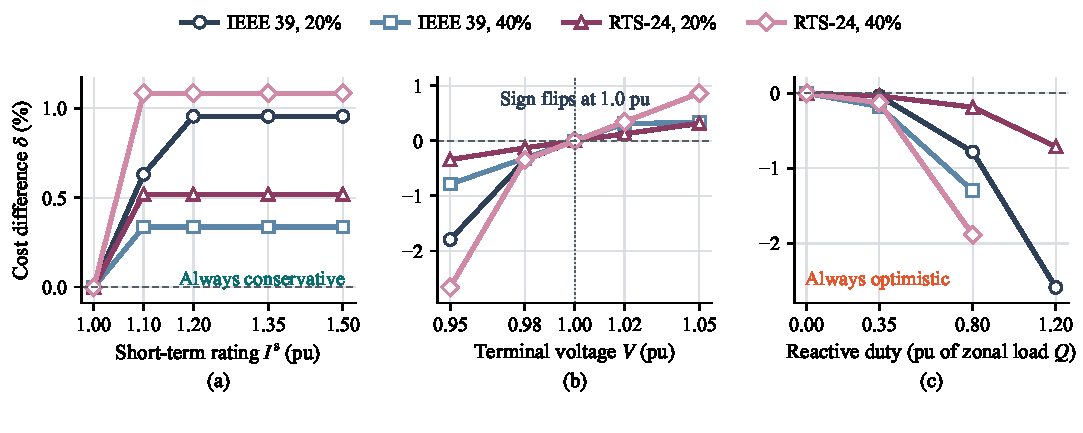
\includegraphics[width=\textwidth]{fig4_sign_flip}
  \caption{$\delta$ for each omitted quantity with the other two removed
  ($e = \SI{0.8}{\pu}$, $m = 192$): (a) short-term rating, (b) terminal
  voltage, (c) reactive requirement as a fraction of zonal reactive load.}
  \label{fig:signs}
\end{figure*}

\subsection{Cost and inertia price}
\label{sec:results-cost}

Table~\ref{tab:rating} gives $\delta$ for the four rating conventions and the
two comparison bounds. The sign is positive in all \num{32} cases. The
magnitude depends on the convention: from \SIrange{0.26}{5.44}{\percent}
with $\bar{P} = S$ and from \SIrange{0.62}{8.25}{\percent} with
$\bar{P} = P^{\mathrm{sch}}$. The sign condition and the direction of the
capability mismatch are therefore properties of the two feasible sets,
whereas the size of the cost difference is conditional on the rating
assumption and should be read with it.

\begin{table}[t]
  \caption{$\delta$ (\%) by converter rating convention and comparison bound
  ($e = \SI{0.8}{\pu}$, $I^{\mathrm{s}} = \SI{1.5}{\pu}$).}
  \label{tab:rating}
  \centering
  \small
  \begin{tabular*}{\columnwidth}{@{\extracolsep{\fill}}ll rr rr@{}}
    \toprule
    & & \multicolumn{2}{c}{IEEE 39} & \multicolumn{2}{c}{RTS-24} \\
    \cmidrule(lr){3-4}\cmidrule(l){5-6}
    $P/S$ & $\bar{P}$ & 0.2 & 0.4 & 0.2 & 0.4 \\
    \midrule
    1.00 & $S = P^{\mathrm{sch}}$ & 1.02 & 0.53 & 0.62 & 5.44 \\
    0.95 & $S$ & 0.98 & 0.41 & 0.67 & 2.67 \\
    0.95 & $P^{\mathrm{sch}}$ & 2.83 & 1.14 & 1.02 & 6.89 \\
    0.90 & $S$ & 0.93 & 0.26 & 0.56 & 1.07 \\
    0.90 & $P^{\mathrm{sch}}$ & 4.85 & 4.49 & 1.67 & 8.25 \\
    reference & $S$ & 0.96 & 0.34 & 0.68 & 1.08 \\
    reference & $P^{\mathrm{sch}}$ & 3.67 & 1.90 & 1.40 & 7.94 \\
    \bottomrule
  \end{tabular*}
\end{table}

\begin{table}[t]
	\caption{$\delta$ (\%) against the active-power bound (AP), apparent-power
		model (S) and uniform derating (UD) at two dispatch levels.}
	\label{tab:ladder}
	\centering
	\small
	\begin{tabular*}{\columnwidth}{@{\extracolsep{\fill}}l rrr rrr@{}}
		\toprule
		& \multicolumn{3}{c}{$e = \SI{0.8}{\pu}$}
		& \multicolumn{3}{c}{$e = \SI{1.0}{\pu}$} \\
		\cmidrule(lr){2-4}\cmidrule(l){5-7}
		System, share & AP & S & UD & AP & S & UD \\
		\midrule
		IEEE 39, 0.2 & 0.96 & 1.01 & 0.93 & 9.00 & 9.38 & 8.82 \\
		IEEE 39, 0.4 & 0.34 & 0.61 & 2.04 & 14.87 & 16.74 & 22.49 \\
		RTS-24, 0.2  & 0.68 & 0.73 & 0.58 & 1.17 & 1.60 & 0.65 \\
		RTS-24, 0.4  & 1.08 & 1.30 & 1.69 & 1.92 & 3.29 & 5.32 \\
		\bottomrule
	\end{tabular*}
\end{table}

The inertia price under the capability set stays within \SI{0.1}{\percent}
of the converter offer, \num{3.0}~\$/MW/h, in every configuration, rating
convention and dispatch level: with the short-term band available, inertial
power is not scarce.
Under Eq.~\eqref{eq:box} inertial power competes with energy for the same
megawatts, and the price rises with converter loading
(Fig.~\ref{fig:cost}a). At $e = \SI{0.8}{\pu}$ it is \numrange{6.75}{8.0}
with $\bar{P} = S$, a ratio of \numrange{2.3}{2.7}, and \numrange{25.6}{41.0}
with $\bar{P} = P^{\mathrm{sch}}$ (reference rating); at
$e = \SI{1.0}{\pu}$ with
$\bar{P} = S$ the ratio is \numrange{7.8}{13.7}. For both models the left and
right limits of the price coincide at perturbations of
\SIlist{1;0.25;0.01}{\MW}, so the price ranges do not overlap and the ratio is
determined; it remains conditional on the illustrative offers, and only its
direction is general. The cost difference also grows with loading: it is zero
at $e = \SI{0.4}{\pu}$ and, at $e = \SI{1.0}{\pu}$, the bound clears at
\num{1.175} times the capability-set cost on IEEE 39-bus
(\SI{40}{\percent} share) and \num{1.020} times on RTS-24, mainly through
replacement energy for curtailed converter output (Fig.~\ref{fig:cost}b).
Curtailment is a primal quantity on a wide optimal face, so it is reported as
a range over that face: on IEEE 39-bus the bound curtails at least
\SI{7243}{\MWh} more than the capability set at every optimum, while on
RTS-24 the two ranges overlap and no difference is claimed.

\begin{figure*}[t]
  \centering
  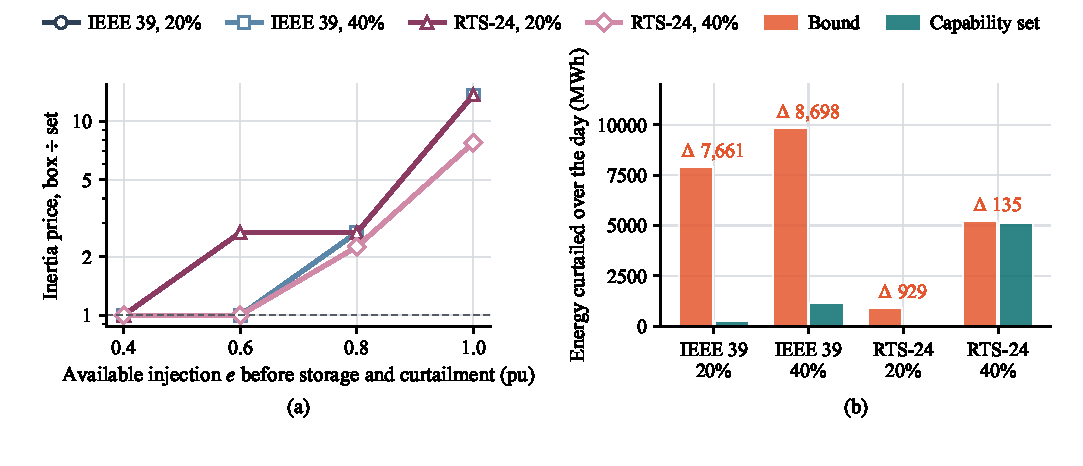
\includegraphics[width=\textwidth]{fig5_price_curtailment}
  \caption{(a) Ratio of the inertia price under the active-power bound
  ($\bar{P} = S$) to that under the capability set against available
  converter injection. (b) Curtailed converter output at
  $e = \SI{1.0}{\pu}$ at the selected optimum.}
  \label{fig:cost}
\end{figure*}

Fig.~\ref{fig:day} follows RTS-24 at \SI{40}{\percent} share through the day.
From the third period the capability set holds at least \SI{43}{\MW} more
converter reserve than the bound, and from the fourth period between
\SI{56.5}{\MW} and \SI{110.4}{\MW} more; these are differences between the
ranges over the two optimal faces, so they hold at every optimum. Under the
capability set the converter reserve is unique in every period, whereas under
the bound its range is about \SI{60}{\MW} wide at the peak. The
state-of-charge trajectories coincide, so the difference is not caused by
storage use.

\begin{figure*}[t]
  \centering
  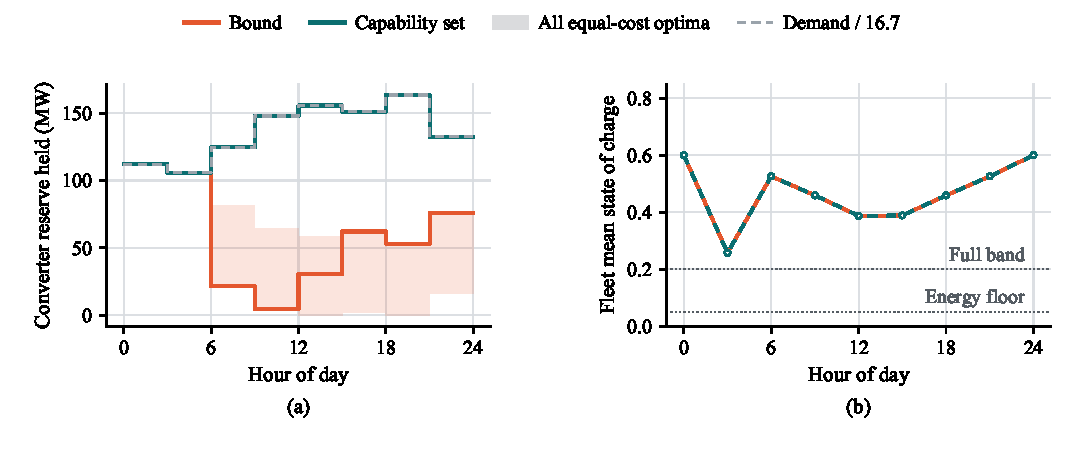
\includegraphics[width=\textwidth]{fig6_day}
  \caption{RTS-24, \SI{40}{\percent} converter share: (a) converter reserve,
  selected optimum (line) and range over the optimal face (band);
  (b) fleet-mean state of charge.}
  \label{fig:day}
\end{figure*}

\subsection{Comparison models, approximation error and generality}
\label{sec:ladder}
\label{sec:sensitivity}
\label{sec:placement}

Table~\ref{tab:ladder} gives $\delta$ against the three comparison models. No
comparison model is cheaper than the capability set in any of the sixteen
combinations of configuration and dispatch; the difference is zero at light
loading and positive otherwise. At full dispatch it is
\SIrange{1.2}{14.9}{\percent} against the active-power bound,
\SIrange{1.6}{16.7}{\percent} against the apparent-power model and
\SIrange{0.6}{22.5}{\percent} against the uniform derating. The uniform
derating keeps every converter within its continuous current, as the
capability set does; the active-power bound does not, and its schedules reach
\SI{1.38}{\pu} of continuous current on RTS-24 (Table~\ref{tab:acfinal},
last column). The
exact second-order cone formulation gives $\delta$ within \num{0.056}
percentage points of the polygon value, and the polygon value is the smaller
in every case, so the reported differences are conservative.

Fig.~\ref{fig:sensitivity} summarises the sensitivity of $\delta$ to the
parameters that a decarbonising system changes. A tighter RoCoF limit, a
lower synchronous inertia constant and a shorter storage duration all
increase $\delta$; at a RoCoF limit of \SI{2}{\hertz\per\second} the inertia
requirement no longer binds on IEEE 39-bus and the two representations
coincide. The offer ratio scales $\delta$ almost proportionally without
changing its sign. The remaining parameters (polygon faces, cycling cost,
reserve overlap, state-of-charge thresholds, terminal-voltage offset) change
$\delta$ by less than \num{0.4} percentage points.

\begin{figure*}[t]
  \centering
  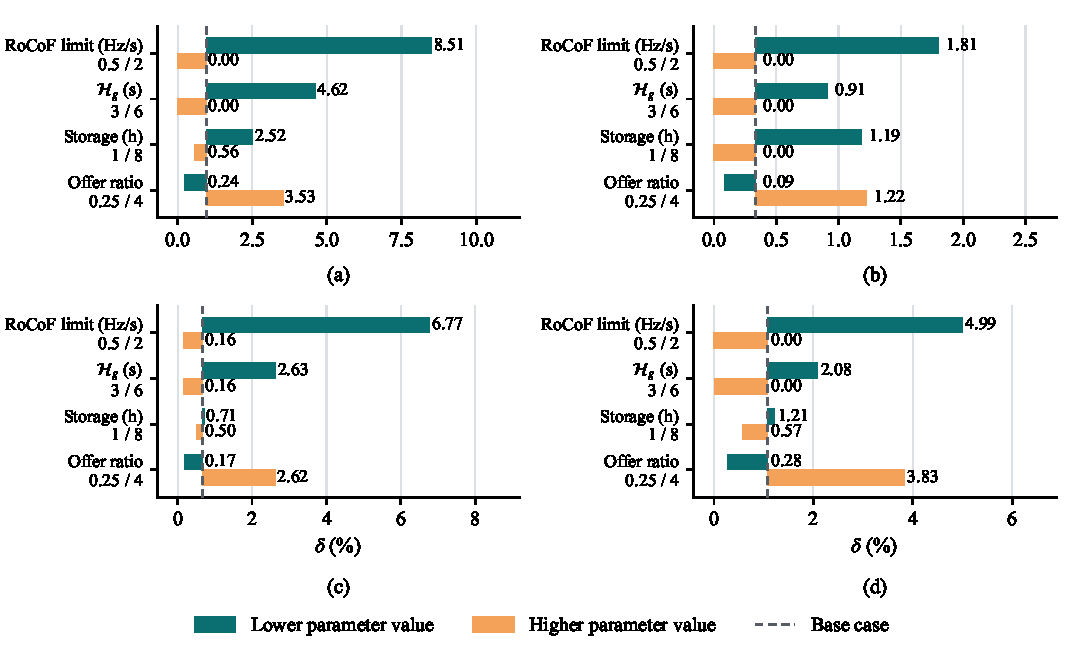
\includegraphics[width=\textwidth]{fig_sensitivity}
  \caption{Sensitivity of $\delta$ to the RoCoF limit, synchronous inertia
  constant, storage duration and offer ratio ($\bar{P} = S$); bars run from
  the base case (dashed) to $\delta$ at the lower and higher parameter value
  given under each label. (a) IEEE 39-bus, \SI{20}{\percent} share, base
  $\delta = \SI{0.96}{\percent}$; (b) IEEE 39-bus, \SI{40}{\percent},
  \SI{0.34}{\percent}; (c) RTS-24, \SI{20}{\percent}, \SI{0.68}{\percent};
  (d) RTS-24, \SI{40}{\percent}, \SI{1.08}{\percent}.}
  \label{fig:sensitivity}
\end{figure*}

\begin{figure}[!tb]
  \centering
  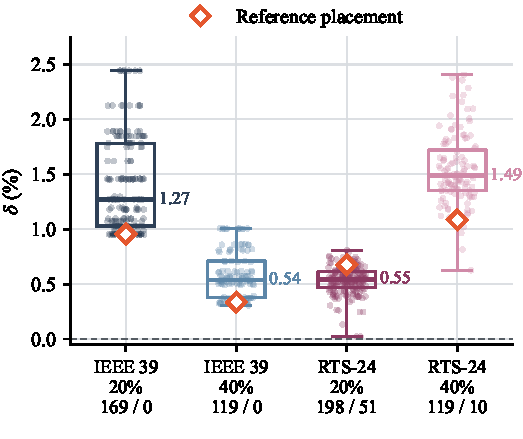
\includegraphics[width=\columnwidth]{fig_placement}
  \caption{$\delta$ over the randomised converter placements: box, quartiles;
  whiskers, range; printed value, median; numbers under each configuration,
  feasible / infeasible draws.}
  \label{fig:placement}
\end{figure}

To test whether the result depends on which units are converters, the
selection was randomised: units are drawn in random order until the capacity
share of the reference placement is reached within \SI{2}{\percent}. Of
\num{666} accepted draws, \num{605} have a feasible clearing, and $\delta > 0$
in all of them (Fig.~\ref{fig:placement}). Within a configuration the
magnitude varies by a factor of \numrange{2.6}{34.5}, and the reference
placement lies in the lower part of the distribution in three of the four
configurations. The \num{61} infeasible draws are all on RTS-24 and are
infeasible under both representations: the zonal reactive requirement cannot
be met with those converter locations. On the IEEE 118-bus system, under the
dc approximation and with $P/S = 0.95$, the inertia requirement binds only at
\SI{40}{\percent} share with a RoCoF limit of \SI{0.5}{\hertz\per\second};
there $\delta = \SI{+0.12}{\percent}$ and the price ratio is \num{2.7}. Where
it does not bind, only the reactive-current omission acts, and $\delta$ is
zero at $e = \SI{0.8}{\pu}$ and \SI{-0.68}{\percent} at full dispatch, the
sign of Fig.~\ref{fig:signs}c. The direction of the
error on a given system thus follows from which constraint binds, as the sign
condition states.

\subsection{AC validation of the final schedules}
\label{sec:results-network}

The procedure of Section~\ref{sec:acloop} was applied to the capability set
and to the active-power bound in all four configurations. All eight final
schedules satisfy the bus voltage, machine reactive, branch loading and
balance limits in an ac power flow (Table~\ref{tab:acfinal}), in
\numrange{5}{13} rounds. The first, lossless clearing leaves \SIrange{32}{76}{\MW}
for the reference machine to supply and loads a branch to at most
\SI{103.2}{\percent}; in the final schedules the reference machine deviates
from its cleared output by less than \SI{1}{\MW} and the largest branch
loading is \SI{99.9}{\percent}. Charging the schedule for its losses raises
the cost by \SIrange{1.0}{2.4}{\percent}. The comparison is unchanged in
sign: $\delta$ is \SIlist{0.85;0.07;0.59;1.00}{\percent} for the ac-feasible
schedules against \SIlist{0.96;0.34;0.68;1.08}{\percent} for the lossless
ones, and the inertia price is \numrange{3.0}{3.03} under the capability set
and \numrange{6.8}{8.5} under the bound. With the converter currents
recomputed at the ac terminal voltages, the capability-set schedules stay at
or below the continuous rating, whereas the schedules of the bound reach
\SIrange{1.34}{1.40}{\pu} on RTS-24.

\begin{table*}[t]
  \caption{AC power-flow validation of the final schedules. Tolerances:
  voltage \SI{e-4}{\pu}, loading \SI{0.05}{\percent}, reactive excess
  \SI{0.5}{\MVAr}, balance \SI{1}{\MW}, converter current \SI{e-3}{\pu}.}
  \label{tab:acfinal}
  \centering
  \small
  \begin{tabular*}{\textwidth}{@{\extracolsep{\fill}}ll r rr r r r r r@{}}
    \toprule
    System, share & Model & Rounds & $V^{\min}$ (pu) & $V^{\max}$ (pu)
      & Loading (\%) & $Q$ exc.\ (MVAr) & Balance (MW)
      & $\Delta$ cost (\%) & $I^{\mathrm{conv}}$ (pu) \\
    \midrule
    IEEE 39, 0.2 & bound & 5 & 0.9432 & 1.0600 & 98.6 & 0.0 & 0.96 & +1.05 & 0.83 \\
    IEEE 39, 0.2 & set & 10 & 0.9400 & 1.0600 & 99.5 & 0.0 & 0.03 & +1.16 & 1.00 \\
    IEEE 39, 0.4 & bound & 6 & 0.9401 & 1.0600 & 94.8 & 0.0 & 0.37 & +1.30 & 1.06 \\
    IEEE 39, 0.4 & set & 6 & 0.9400 & 1.0600 & 95.2 & 0.0 & 0.55 & +1.57 & 1.00 \\
    RTS-24, 0.2 & bound & 6 & 0.9650 & 1.0500 & 86.7 & 0.0 & 0.64 & +1.38 & 1.34 \\
    RTS-24, 0.2 & set & 9 & 0.9588 & 1.0500 & 97.3 & 0.0 & 0.05 & +1.47 & 1.00 \\
    RTS-24, 0.4 & bound & 5 & 0.9556 & 1.0500 & 99.7 & 0.0 & 0.20 & +2.31 & 1.40 \\
    RTS-24, 0.4 & set & 13 & 0.9558 & 1.0481 & 99.9 & 0.0 & 0.00 & +2.40 & 1.00 \\
    \bottomrule
  \end{tabular*}
\end{table*}

\subsection{Post-contingency deliverability}
\label{sec:postcontingency}

Equation~\eqref{eq:secure} was imposed for the synchronous units with the
largest active limits (five to eight per configuration). Without it, the
response model of Section~\ref{sec:secure-form} overloads a branch beyond its
emergency rating in up to \num{29} of \num{47} secured outage--period cases,
with a worst loading of \SI{129}{\percent}. With it, the worst loading is
\SIrange{100.0}{100.1}{\percent} in all eight clearings, the cleared cost
rises by at most \SI{0.06}{\percent}, the inertia and reserve prices are
unchanged, and $\delta$ is unchanged except on RTS-24 at \SI{40}{\percent}
share, where it moves from \SI{1.09}{\percent} to \SI{1.14}{\percent}
(Table~\ref{tab:secured}). The results of Sections~\ref{sec:results-cost}
and~\ref{sec:ladder} therefore hold when the procured response is required
to be deliverable after the critical outages. Outages outside the secured set
are screened but not constrained.

\begin{table}[t]
  \caption{Post-contingency deliverability for the secured generator outages:
  worst branch loading relative to the emergency rating without and with
  Eq.~\eqref{eq:secure}, and cost increase.}
  \label{tab:secured}
  \centering
  \small
  \begin{tabular*}{\columnwidth}{@{\extracolsep{\fill}}ll r rr r@{}}
    \toprule
    & & & \multicolumn{2}{c}{Worst loading (\%)} & Cost \\
    \cmidrule(lr){4-5}
    System, share & Model & $|\Omega|$ & without & with & (\%) \\
    \midrule
    IEEE 39, 0.2 & bound & 7 & 113.9 & 100.0 & 0.00 \\
    IEEE 39, 0.2 & set & 7 & 129.2 & 100.1 & 0.00 \\
    IEEE 39, 0.4 & bound & 5 & 109.2 & 100.0 & 0.00 \\
    IEEE 39, 0.4 & set & 5 & 122.9 & 100.0 & 0.00 \\
    RTS-24, 0.2 & bound & 8 & 97.0 & 97.0 & 0.00 \\
    RTS-24, 0.2 & set & 8 & 90.1 & 90.1 & 0.00 \\
    RTS-24, 0.4 & bound & 7 & 105.6 & 100.0 & 0.06 \\
    RTS-24, 0.4 & set & 7 & 107.6 & 100.0 & 0.00 \\
    \bottomrule
  \end{tabular*}
\end{table}

\subsection{Dynamic verification of the short-term constraint}
\label{sec:results-dynamic}
\label{sec:applied}

Whether a converter delivers the scheduled inertial power within its current
limit was tested with an RMS model of one GFM converter: a virtual
synchronous machine behind a filter reactance, connected through a reactance
$x^{\mathrm{g}}$ to a Th\'evenin source, with a current limiter that applies
the two ratings and the priority rule of Eq.~\eqref{eq:short} and an
anti-windup clamp (Supplementary Section~S8). The virtual inertia is set so
that the scheduled $H_i$ is requested at the design RoCoF of
\SI{1}{\hertz\per\second}. The \num{360} runs combine $V \in \{0.95, 1.00,
1.05\}$~pu, low and high reactive schedules and the crossing
$\tilde{Q}^{\mathrm{crit}}$ (conservative, crossing and optimistic regions of
the Proposition), $I^{\mathrm{s}} \in \{1.1, 1.5\}$~pu, reactive and active
priority, $x^{\mathrm{g}} \in \{0.05, 0.15, 0.30\}$~pu, and a grid voltage
that is either constant or falls by \SI{5}{\percent} at the event.

The limiter becomes active in all runs, \SIrange{0.07}{0.34}{\second} after
the event, and the converter current does not exceed the limit in force
(Fig.~\ref{fig:dynamic}, Table~\ref{tab:dynamic}). In every run the settled active power equals the
boundary of Eq.~\eqref{eq:short} evaluated at the terminal voltage reached
during the event. The shortfall against the schedule is therefore a voltage
effect. With the grid voltage constant, the terminal voltage falls by
\SIrange{0.06}{0.25}{\percent} for $x^{\mathrm{g}} = \SI{0.05}{\pu}$ and the
converter delivers \SIrange{99.5}{99.7}{\percent} of the scheduled inertial
power; for $x^{\mathrm{g}} = \SI{0.15}{\pu}$ the figures are
\SIrange{0.5}{2.3}{\percent} and \SIrange{95.1}{97.7}{\percent}; for
$x^{\mathrm{g}} = \SI{0.30}{\pu}$ the voltage falls by up to
\SI{9.5}{\percent} and delivery is \SI{79.9}{\percent} in the worst case. With
the grid voltage falling by \SI{5}{\percent} the worst case is
\SI{54.0}{\percent}. Delivery correlates with $x^{\mathrm{g}}$ ($-0.93$) and
not with the region of the Proposition. Under voltage-droop reactive control
the converter holds its terminal voltage at the expense of active current,
and in \num{16} of \num{90} droop runs with falling grid voltage the active
response is lost; the constraint assumes that the reactive schedule is held,
as Eq.~\eqref{eq:priority} states.


The pre-contingency voltage is thus not a safe value for the short-term
constraint at weak buses, and the constraint is corrected rather than its
coefficients. With the reactive schedule held, the terminal voltage during
the event follows from the reactance behind the terminal,
%
\begin{equation}
  \bigl(V^{\mathrm{sh}}_i\bigr)^2 = V_i^2 - \bigl(x^{\mathrm{g}}_i\bigr)^2
    \left[ \bigl(I^{\mathrm{s}}\bigr)^2 - I_i^2 \right] ,
  \label{eq:shortvoltage}
\end{equation}
%
with $I_i$ the pre-event current; it reproduces the simulated voltages to
numerical precision. The reactance $x^{\mathrm{g}}_i$ is obtained from the
voltage sensitivities of Section~\ref{sec:acloop}. Using
$V^{\mathrm{sh}}_i$ in Eq.~\eqref{eq:short} lowers the short-term face by up
to \SI{12.4}{\percent} (IEEE 39-bus, \SI{40}{\percent} share). Re-clearing
with the corrected face leaves the cost and the total scheduled inertial
power unchanged and reallocates the inertial obligation between converters.
When the corrected schedules are passed through the converter model, the
energy delivered in the containment window, weighted by scheduled inertial
power, changes from \SI{86.3}{} to \SI{89.9}{\percent} and from \SI{80.7}{} to
\SI{83.4}{\percent} on IEEE 39-bus, and from \SI{92.8}{} to
\SI{93.3}{\percent} and from \SI{97.7}{} to \SI{97.0}{\percent} on RTS-24; the
tenth percentile rises from \SI{54.0}{} to \SI{75.9}{\percent} where it was
lowest. The remaining shortfall is the rise time of the response, which
depends on the virtual inertia and damping and not on the capability set.

\begin{table}[t]
	\caption{RMS verification with the reactive schedule held and constant grid
		voltage: delivered inertial power (\% of schedule), terminal-voltage drop
		and time of limiter activation.}
	\label{tab:dynamic}
	\centering
	\small
	\begin{tabular*}{\columnwidth}{@{\extracolsep{\fill}}l r rrr@{}}
		\toprule
		Region ($I^{\mathrm{s}}$) & $x^{\mathrm{g}}$ (pu) & Delivered (\%)
		& $\Delta V$ (\%) & $t^{\lim}$ (s) \\
		\midrule
		Conservative & 0.05 & 99.5--99.7 & 0.1--0.3 & 0.12--0.17 \\
		(1.5 pu) & 0.15 & 95.1--97.7 & 0.9--2.3 & 0.17--0.25 \\
		& 0.30 & 79.9--90.6 & 3.5--9.5 & 0.23--0.34 \\
		Crossing & 0.05 & 99.6--99.7 & 0.1 & 0.10--0.11 \\
		(1.1 pu) & 0.15 & 96.8--97.4 & 0.6--0.9 & 0.15--0.17 \\
		& 0.30 & 86.9--89.3 & 2.4--3.6 & 0.21--0.23 \\
		Optimistic & 0.05 & 99.5--99.7 & 0.1 & 0.08--0.10 \\
		(1.1 pu) & 0.15 & 95.8--97.3 & 0.5--0.6 & 0.12--0.15 \\
		& 0.30 & 82.9--89.1 & 2.1--2.3 & 0.17--0.21 \\
		\bottomrule
	\end{tabular*}
\end{table}



\begin{figure*}[t]
  \centering
  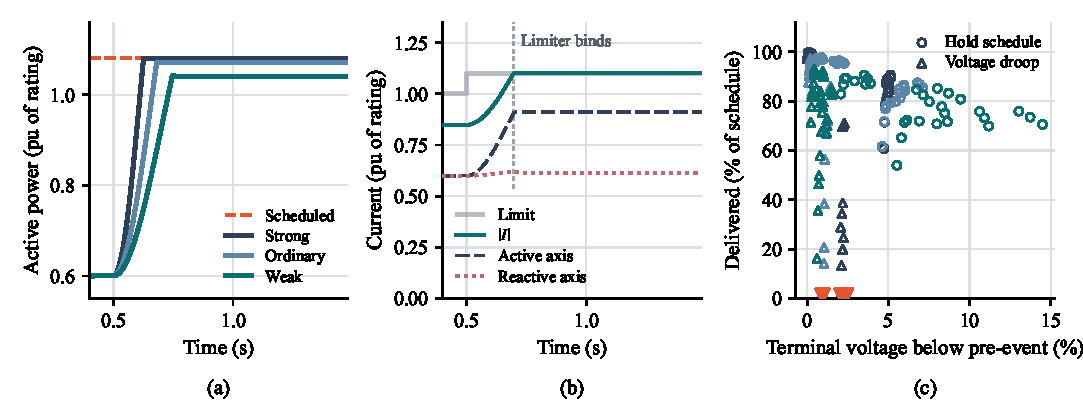
\includegraphics[width=\textwidth]{fig_dynamic}
  \caption{RMS verification: (a) active power for three grid reactances
  against the schedule; (b) current magnitude, limit and axis currents for
  $x^{\mathrm{g}} = \SI{0.30}{\pu}$; (c) delivered against scheduled inertial
  power versus terminal-voltage drop, all \num{360} runs.}
  \label{fig:dynamic}
\end{figure*}

\section{Conclusion}
\label{sec:conclusion}

The active-power bound used in shared-capability scheduling is the projection
of the converter current limit onto zero reactive power at unit voltage
without a short-term rating. This paper replaced it by a polyhedral
capability set with continuous and short-term current ratings, reactive
current and terminal voltage, in a multi-period linear clearing of energy,
reserve and inertia, and derived a piecewise condition for the sign of the
error of the bound. The condition depends on the short-term radius, the bound
and the reactive current held during the response. In the clearing, the
three omissions produce errors of different sign (\SIrange{0}{+1.1}{\percent},
\SIrange{-2.7}{+0.9}{\percent} and \SIrange{-2.6}{0}{\percent} of cost), so
the bound cannot be corrected by a constant factor.

On the IEEE 39-bus and RTS-24 systems the capability set was never more
expensive than the active-power bound, the apparent-power model or a safe
uniform derating, in \num{32} rating and bound conventions and \num{605}
randomised placements. The cost difference is about \SI{1}{\percent} at the
base case, up to \SI{8.5}{\percent} with a tighter RoCoF limit and
\SIrange{0.6}{22.5}{\percent} at full converter dispatch; its size depends on
the rating convention and on the offers. The capability set prices inertial
power at the converter offer, while the bound prices it
\numrange{2.3}{13.7} times higher depending on loading and bound. All final
schedules satisfy voltage, machine reactive, branch and balance limits in an
ac power flow, the results hold when the response is constrained to be
deliverable after the largest generator outages, and an RMS converter model
delivers the scheduled inertial power within the current limit at the
terminal voltage reached during the event, for which a closed-form correction
of the short-term constraint was given.

The limitations fall into four groups. \emph{Network and ac feasibility:} the
final schedules are ac-feasible for the pre-contingency state, and prices are
those of the final linearised subproblem; post-contingency security covers
generator outages with a shift-factor model and an emergency rating, not
branch outages or post-contingency voltages. \emph{Converter dynamics:} the
verification uses one converter in RMS without inner loops, dc-link dynamics,
fault current or ride-through logic, and corrected short-term voltages as low
as \SI{0.88}{\pu} would engage such functions; an electromagnetic-transient
study on a network is needed. \emph{Market and pricing assumptions:}
commitment is fixed, offers are illustrative and identical within a
technology, and the contingency is taken at the scheduled bound of each unit;
no absolute price should be read from the results. \emph{Scale and data:}
the study uses two benchmark systems and an additional 118-bus check;
behaviour on an operator model, optimised siting and dc-side power limits
remain for further work.


\section*{CRediT authorship contribution statement}

\textbf{Junseok Lim:} Conceptualization, Methodology, Software, Validation,
Formal analysis, Writing -- original draft. \textbf{Sanghyuk Ji:} Validation,
Investigation, Writing -- review \& editing. \textbf{Byungjun Lee:}
Validation, Visualization, Writing -- review \& editing. \textbf{Sungwoo
Bae:} Supervision, Funding acquisition, Writing -- review \& editing.

\section*{Declaration of competing interest}

The authors declare that they have no known competing financial interests or
personal relationships that could have appeared to influence the work
reported in this paper.

\section*{Data availability}

The code, the modified test cases and converter mapping, the parameters, the
result files behind every table and figure, and the scripts that regenerate
them are available at
\url{https://github.com/Junseok-Lim-HY/gfm-capability-set-clearing}.
% On acceptance: make the repository public, create the Zenodo release and
% append "and archived at https://doi.org/10.5281/zenodo.XXXXXXX".

\section*{Funding}

This work was supported by the Korea Institute of Energy Technology Evaluation and Planning (KETEP) and the Ministry of Climate, Energy and Environment (MCEE) of the Republic of Korea (RS-2023-00234563, Development of power system modeling \& analysis and interoperability evaluation technology applied with grid forming based on distributed energy; and RS-2024-00422103, EV Smart Charging Platform Innovation Research Center).

\bibliographystyle{elsarticle-num}
\bibliography{refs}

\end{document}
